\pgfplotsset{grid style={dashed}}
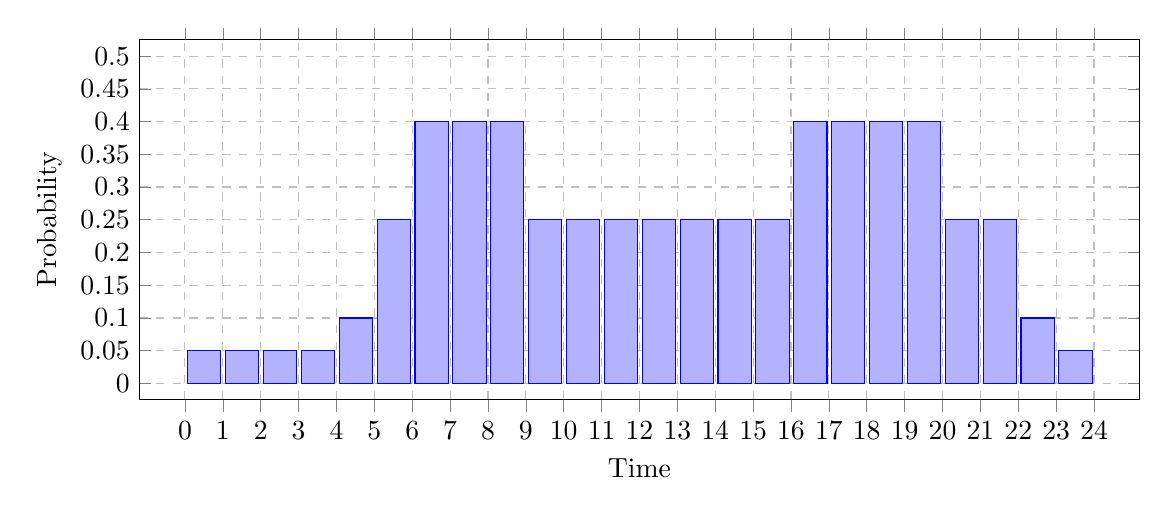
\begin{tikzpicture}
\begin{axis}[grid=major,
scale only axis,
    ybar,
    bar shift=7pt,
    bar width=12pt,
    width=5in,height=1.8in,
    ymin=0.0,ymax=0.50 ,
    xmin=0, xmax=24,
    enlargelimits=0.05,
    ylabel={Probability},
    xlabel={Time},
    symbolic x coords={0,1,2,3,4,5,6,7,8,9,10,11,12,13,14,15,16,17,18,19,20,21,22,23,24},
    xtick={0,1,...,24},
    ytick={0,0.05,...,0.5},
    %nodes near coords,
    nodes near coords align={vertical},
    y tick label style={/pgf/number format/.cd,%
              scaled y ticks = false,
              set thousands separator={},
              fixed,},
    ]
\addplot coordinates {
(0,0.05)
(1,0.05)
(2,0.05)
(3,0.05)
(4,0.1)
(5,0.25)
(6,0.4)
(7,0.4)
(8,0.4)
(9,0.25)
(10,0.25)
(11,0.25)
(12,0.25)
(13,0.25)
(14,0.25)
(15,0.25)
(16,0.4)
(17,0.4)
(18,0.4)
(19,0.4)
(20,0.25)
(21,0.25)
(22,0.1)
(23,0.05)
};
\end{axis}
\end{tikzpicture}
